\chapter{Quantum walk}

Classical random graph walks can be seen as using a classical coin flip to decide in the current vertex which neighbouring vertex to step next. To create a quantum version of these walks, we define the quantum coin to randomize the walk, then use entanglement between the coin and the register of the current vertex, to influence stepping.

A great introduction to quantum walks is in Portugal's Quantum Walks and Search Algorithms book \cite{Portugal}.

\section{Definition of the quantum coin}

The quantum coin has a current state, which according to Postulate 1 and 4 is an n-qubit register and a transition operator, which according to Postulate 2 is a unitary matrix.

The current state decides where to step next. If there are $d$ neighbours to choose from, the coin's current state register must be $d$ dimensional.

The transition operator decides how the coin is flipped. If the coin is $d$ dimensional, the transition operator is a $d\times{}d$ dimensional matrix. Based on what the transition operator is, multiple types of coins can be defined. The following ones are typically used in quantum walks.

\definition{\textbf{Hadamard coin}}

The Hadamard coin uses the Hadamard-matrix as a transition operator, which is the following:

\begin{align}
  H = \frac{1}{\sqrt{2}}\begin{pmatrix}
      1 & 1  \\
      1 & -1
    \end{pmatrix}
\end{align}

If the starting coin state is $\ket{0}$, then flipping the coin once results in the following state:

\begin{align}
 H\ket{0} = \frac{1}{\sqrt{2}}\begin{pmatrix}
      1 & 1  \\
      1 & -1
    \end{pmatrix} \begin{pmatrix} 1 \\ 0 \end{pmatrix}
    = \frac{1}{\sqrt{2}} \begin{pmatrix} 1 \\ 1 \end{pmatrix} = \frac{1}{\sqrt{2}} \ket{0} + \frac{1}{\sqrt{2}} \ket{1}
\end{align}

If we measured the above coin, the probability of measuring $\ket{0}$ is $\left\lvert\frac{1}{\sqrt{2}}\right\rvert^2 + \left\lvert\frac{1}{\sqrt{2}}\right\rvert^2 = \frac{1}{2}$.

Similarly the starting coin state is $\ket{1}$, then flipping the coin once results in the following state:

\begin{align}
   H\ket{1} = \frac{1}{\sqrt{2}}\begin{pmatrix}
      1 & 1  \\
      1 & -1
    \end{pmatrix} \begin{pmatrix} 0 \\ 1 \end{pmatrix}
    = \frac{1}{\sqrt{2}} \begin{pmatrix} 1 \\ -1 \end{pmatrix} = \frac{1}{\sqrt{2}} \ket{0} - \frac{1}{\sqrt{2}} \ket{1}
\end{align}

the probability of measuring $\ket{1}$ is similarly $\left\lvert\frac{1}{\sqrt{2}}\right\rvert^2 + \left\lvert-\frac{1}{\sqrt{2}}\right\rvert^2 = \frac{1}{2}$.

An interesting property about this coin is related to the fact, that the Hadamard-matrix is Hermitian (self-adjoint), i.e. $H^{\dagger} = H$, while also unitary, i.e. $H^{\dagger} = H^{-1}$, which results in $H^{-1} = H$, thus $HH = I$. This means, that if we flip the coin twice, without measuring it, it will return to its original state, for example:

\begin{align}
 H^2 \ket{0} = H\frac{1}{\sqrt{2}}(\ket{0} + \ket{1}) = \frac{1}{2}(\ket{0} + \ket{1} + \ket{0} - \ket{1}) = \ket{0}
\end{align}

After the second flip, the probability of measuring $\ket{0}$ is 1, due to the destrutive interference between the $\ket{1}$ vectors. This illustrates the vast difference between classical and quantum walks.

\definition{\textbf{$2^n$ dimensional Hadamard-coin}}: A $2^n$ dimensional Hadamard-coin can be created by taking the tensor product of the $2$ dimensional Hadamard-coin $n$ times: $H^{\otimes{}n}$



\definition{\textbf{Grover coin}}

The Grover coin's origin is the Grover search algorithm, where it is used as the diffusion operator, defined as follows:

The diagonal state of the coin space:

\begin{align}
    \ket{D} = H^{\otimes{}n}\ket{0} = \frac{1}{\sqrt{2^n}} \sum\limits_{i=0}^{2^n-1} \ket{i}
\end{align}

Grover coin:

\begin{align}
    G = 2\ket{D}\bra{D} - I
\end{align}

If $N = 2^n$, then

\begin{align}
  G = \begin{pmatrix}
      \frac{2}{N} - 1 & \frac{2}{N} & \dots  & \frac{2}{N} \\
      \frac{2}{N} & \frac{2}{N} - 1 & \dots  & \frac{2}{N} \\
      \vdots & \vdots & \ddots & \vdots \\
      \frac{2}{N} & \frac{2}{N} & \ddots & \frac{2}{N} - 1
    \end{pmatrix}
\end{align}

\paragraph{Fourier coin}

While both the Hadamard and the Fourier coin need to be sized as a power of $2$, the Fourier coin does not have this limitation. A size $N$ Fourier-coin, $F_N$ is defined by the matrix of the Fourier-transform:

\unsure{A Quanutm diszkrét Fourier transzformáció mátrixa talán ez?}

\begin{align}
[F_N]_{k,l} = \frac{1}{\sqrt{N}} \omega^{kl}
\end{align}

where 
\begin{align}
    \omega = e^{\frac{2\pi{}i}{N}}
\end{align}

\begin{align}
  F_N = \frac{1}{\sqrt{N}}\begin{pmatrix}
      1 &  1 & \dots  & 1 \\
      1 &  e^{\frac{2\pi{}i}{N}} & \dots  & e^{\frac{2\pi{}i(N-1)}{N}} \\
      \vdots & \vdots & \ddots & \vdots \\
      1 &  e^{\frac{2\pi{}i(N-1)}{N}} & \ddots & e^{\frac{2\pi{}i(N-1)^2}{N}}
    \end{pmatrix}
\end{align}

\section{Quantum walks on the line}

\change{Ez félig az önlabomból van és a Kempe cikkből, gondoltam picit rövidítve be lehetne tenni ide.}
\change{Az önlabomat lehet fel kellene töltenem valahova, ha már hivatkozok rá.}

The simplest form of a quantum walk to discuss is the quantum walk on the line. A great introduction into this is in \cite{KempeIntroduction}. In this type of walk, a particle is described by its position on the line $\ket{x}$ and its spin state $\ket{s}$.

The spin state is a $2$-dimensional Hilbert space $H_2$ and the basis states are called spin up $\ket{s} = \ket{\uparrow} = \ket{0}$ or a spin down $\ket{s} = \ket{\downarrow} = \ket{1}$. Let us state, that at the start of the walk, the particle is at the origin, $\ket{0}$ and the walking lasts for $\ket{N}$ steps. Then, the position state is a $(2N+1)$-dimensional Hilbert space $H_{(2N+1)}$ with basis vectors $\{\ket{-N},\ket{-(N-1)},\dots,\ket{-1},\ket{0},\ket{1},\dots,\ket{N-1},\ket{N}\}$ corresponding to the possible positions on the line.

\unsure{Itt nem tudom eldönteni, hogy negatív számokat használjak vagy N/2-ből induljon a részecske és ne 0-ból.}

The complete state of the system, according to the 4th Postulate is $\ket{x}\otimes{}\ket{s}$.

The particle travels on the line based on its current spin state. If the current spin state is $\ket{0}$, the particle moves to the left, i.e. from position $\ket{i}$ the particle travels to position $\ket{i-1}$ $\forall -N < i$ and stays in $\ket{-N}$ for $i=-N$. If the current spin state is $\ket{1}$, the particle moves to the right, i.e. from position $\ket{i}$ the particle travels to position $\ket{i+1}$ $\forall i<N$ and stays in $\ket{N}$ for $i=N$.

This step is described by the unitary matrix $S$, which operates on the complete state of the system, $\ket{x}\otimes{}\ket{s}$ and is constructed as follows:

\change{Cite this?}

\definition{\textbf{Kronecker delta}} Kronecker delta is a function acting on two input variables, which takes the output value $1$, when the input variables equal and the output value $0$, when the input variables differ.

\begin{align}
    \delta_{i,j} =
    \begin{cases}
      1 & \text{if $i=j$}  \\
      0 & \text{if $i\neq{}j$}
    \end{cases}
  \end{align}

Using the Kronecker delta function, a matrix can be defined with the following notation:

\begin{align}
    M = [\delta_{f(i),g(j)}]_{i,j}
\end{align}

which means

\begin{align}
M_{i,j} = \delta_{f(i),g(j)}
\end{align}

\change{Ezt valahogy szebben kellene írni.}
To simplify notation, $f(i)$ and $g(j)$ are interpreted with a modulo operator of the size of the matrix.

\definition{\textbf{Left shift operator}}

To move from position $\ket{x}$ to the left, $\ket{x}$ is multiplied with a matrix of size $(2N+1)\times(2N+1)$, that contains $1$'s above the diagonal and in the lower left corner, as follows:

\begin{center}
  \[ L = [\delta_{(i+1),j}]_{i,j}
    \left(
    \begin{array}{ccccc}
        0      & 1      & 0      & \cdots & 0      \\
               & \ddots & \ddots & \ddots & \vdots \\
        \vdots &        & \ddots & \ddots & 0      \\
               &        &        & \ddots & 1      \\
        1      &        & \cdots &        & 0
      \end{array}
    \right)
  \]
\end{center}

\definition{\textbf{Right shift operator}}

To move from position $\ket{x}$ to the right, $\ket{x}$ is multiplied with a matrix of size $(2N+1)\times(2N+1)$, that contains $1$'s below the diagonal and in the upper right corner, as follows:

\begin{center}
  \[ U = [\delta_{(i-1),j}]_{i,j}
    \left(
    \begin{array}{ccccc}

        0      &        & \cdots &        & 1      \\
        1      & \ddots &        &        &        \\
        0      & \ddots & \ddots &        & \vdots \\
        \vdots & \ddots & \ddots & \ddots &        \\
        0      & \cdots & 0      & 1      & 0
      \end{array}
    \right)
  \]
\end{center}

\paragraph{Shift operator}

Using matrixes $L$ and $U$ operating on the position register $\ket{x}$ only, we construct a unitary operator $S$, which operates on the complete state of the system, $\ket{x} \otimes \ket{s}$, executing matrix $L$ on $\ket{x}$ only when $\ket{s} = \ket{0}$ and matrix $U$ only when $\ket{s}=\ket{1}$.

The operator is the following:

\begin{align}
  S = L\otimes\ket{0}\bra{0} + U\otimes\ket{1}\bra{1}
\end{align}

The execution logic is as follows:

\change{TODO: tenzorszorzás disztributivitását kellene itt szépen behivatkozni.}

(Let us assume that the position is not $\ket{-N}$ or $\ket{N}$ for simplicity.)
\change{TODO: |x-1> nem mindig megy balra, ezt hogy kellene jelölni 3.18-ra?}

\begin{align}
    S(\ket{x}\otimes{}\ket{s}) = \\
    (L\otimes\ket{0}\bra{0} + U\otimes\ket{1}\bra{1})(\ket{x}\otimes{}\ket{s}) = \\
    (L\otimes\ket{0}\bra{0})(\ket{x}\otimes{}\ket{s}) + (U\otimes\ket{1}\bra{1})(\ket{x}\otimes{}\ket{s}) = \\
    L\ket{x}\otimes(\ket{0}\bra{0}\ket{s}) + U\ket{x}\otimes(\ket{1}\bra{1}\ket{s}) = \\
    \ket{x-1}\otimes{}s_0\ket{0} + \ket{x+1}\otimes{}s_1\ket{1}
\end{align}

If the spin state was $\ket{s} = \ket{0}$ at the beginning, then $s_1=0$, which means the resulting system state is $\ket{x-1}\otimes{}\ket{0}$, which means the particle shifted to the left, as designed. If the spin state was $\ket{s} = \ket{1}$ at the beginning, then $s_0=0$, which means the resulting system state is $\ket{x+1}\otimes{}\ket{1}$, which means the particle shifted to the right, also as intended.

However the spin state can be any mixed state as well. This means, for a mixed spin state, the particle will shift both to the left and to the right, at the same time. When measured, the particle can be found in position $\ket{x-1}$ with probability $|s_0|^2$ and in $\ket{x+1}$ with probability $|s_1|^2$.

In quantum graph walks, the walker can simultaneously explore multiple parallel paths in the graph, at the same time. With good design, this behaviour can be used to search the graph faster than in classical random graph walks.

\unsure{Itt be lehetne rakni azokat a nagy mátrix ábrákat az önlabomból, vagy csak hivatkozni, vagy inkább semmit.}

\paragraph{Coin operator}

To introduce randomness into the walk, between each step, the particle's spin state is transformed using any $2$ dimensional unitary matrices. The reviously mentioned Hadamard, Grover or Fourier coins are commonly used as coin operators.

For any $U_c$ unitary coin flip transform on the coin register, the coin operator for the complete system is defined as follows:

\begin{align}
    C = I \otimes U_c
\end{align}

since the coin operator does not modify the position register.

\paragraph{Complete step}

One step of the quantum walk on the line consists of flipping the coin once, then applying the shift operator, as follows:

\begin{align}
    U = SC = S(I\otimes{}U_c)
\end{align}

\paragraph{Measurement}

To measure the probability of the particle being at position $\ket{i}$, the projective measurement operator acting on $\ket{x}$ is defined as $P_i = \ket{i}\bra{i}$, according to the projective measurement definition previously.

\change{Behivatkozni hogyan kell?}

Since the coin register need not be measured, we apply the identity operator on it, using $P_i \otimes I$ on the complete system to measure the particle's current position.

The probability of finding the particle in position $i$ is:

\begin{align}
    P(i | \ket{x}) = \bra{x,s}P_i\otimes{}I\ket{x,s}
\end{align}

\section{Kvantumséta a rácson}

A következőkben a rácson, mint 4-reguláris gráfon vett bolyongást fogjuk
részletesen megvizsgálni.

Legyen a rács $N = n \times n$ -es.

Pozíció vektor: $\ket{P} =  (p_{0}, \dots, p_{N})$, ahol
$p_{i}\in\mathds{C}$ ahol $0 \leq{} i < N$, $\forall{}i$-re és $\sum\limits_{i=0}^{N} |p_i|^2 = 1$.

\begin{align}
  \ket{P_{0}} =  (0, \dots, 0, 1, 0, \dots, 0)
\end{align}

\begin{align}
  C = (\frac{1}{\sqrt{2}}, \frac{i}{\sqrt{2}}) \otimes (\frac{1}{\sqrt{2}}, \frac{i}{\sqrt{2}})
\end{align}

\begin{align}
  S_{\text{left}} =
  \begin{pmatrix}
    0      & 0      & 0      & \dots  & 0 \\
    1      & 0      & 0      & \dots  & 0 \\
    0      & 1      & 0      & \ddots & 0 \\
    \vdots & \ddots & \ddots & 0
  \end{pmatrix}
\end{align}

% https://hu.wikipedia.org/wiki/Kronecker_delta_f%C3%BCggv%C3%A9ny
\begin{definition}[Kronecker delta]
  Olyan kétváltozós függvény ami akkor $1$, ha a két változója egyenlő, egyébként $0$.
  \begin{align}
    \delta_{ij} =
    \begin{cases}
      0 & \text{ha $i\neq{}j$} \\
      1 & \text{ha $i=j$}
    \end{cases}
  \end{align}
\end{definition}

% https://en.wikipedia.org/wiki/Shift_matrix
\begin{definition}[Upper cyclic shift matrix]
  Az $U_{k}$ mátrix egy olyan ($k\times{}k$)-s mátrix, aminek a felső mellékátlóján és a bal alsó sarokban
  $1$-esek vannak, máshol $0$-k.
  Az index számozása moduló k történik.
  Ennek az $i$. sor, $j$. oszlopában:
  \begin{align}
    U_{k}[i,j] = \delta_{(i+1),j}
  \end{align}
\end{definition}

\begin{definition}[Lower cyclic shift matrix]
  Az $L_{k}$ mátrix egy olyan ($k\times{}k$)-s mátrix, aminek az alsó mellékátlóján és a jobb felső sarokban
  $1$-esek vannak, máshol $0$-k.
  Az index számozása moduló k történik.
  Ennek az $i$. sor, $j$. oszlopában:
  \begin{align}
    L_{k}[i,j] = \delta_{i,j+1}
  \end{align}
\end{definition}

\begin{align}
  L = U^{T}
\end{align}


\begin{itemize}
  \item Rács = két körnek a tenzorszorzata.
  \item Fel/le = mindig 1 sorral felette/alatta lévő (modulóval) van összekötve = n-el van elcsúsztatva.
  \item Függőlegesen számozva ugyanígy csak fordított elnevezések.
  \item Jobbra-balra = 1 távolság, kivéve sor végén, ahol a sor elejére ugrik = kis körök.
  \item Tenzorszorzás tulajdonságait előre kiszedni, műveletek, használatkor hivatkozni.
  \item Többsoros képleteknek csak 1 száma legyen.
\end{itemize}

\section{Példa}

\begin{align}
  n = 3
\end{align}

\begin{figure}[!ht]
  \begin{center}
    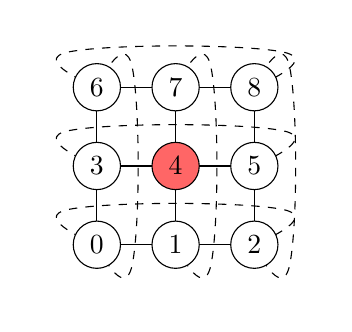
\begin{tikzpicture}

      \draw(0,0) -- (0,2);
      \draw(1,0) -- (1,2);
      \draw(2,0) -- (2,2);

      \draw [black, dashed] plot [smooth, tension=0.8] coordinates { (0,0) (0.45,-0.25) (0.45,2.25) (0,2)};
      \draw [black, dashed] plot [smooth, tension=0.8] coordinates { (1,0) (1.45,-0.25) (1.45,2.25) (1,2)};
      \draw [black, dashed] plot [smooth, tension=0.8] coordinates { (2,0) (2.45,-0.25) (2.45,2.25) (2,2)};


      \draw(0,0) -- (2,0);
      \draw(0,1) -- (2,1);
      \draw(0,2) -- (2,2);

      \draw [black, dashed] plot [smooth, tension=0.8] coordinates { (0,0) (-0.35,0.45) (2.35,0.45) (2,0)};
      \draw [black, dashed] plot [smooth, tension=0.8] coordinates { (0,1) (-0.35,1.45) (2.35,1.45) (2,1)};
      \draw [black, dashed] plot [smooth, tension=0.8] coordinates { (0,2) (-0.35,2.45) (2.35,2.45) (2,2)};

      \draw[black,fill=white](0,0) circle (0.3) node {0};
      \draw[black,fill=white](1,0) circle (0.3) node {1};
      \draw[black,fill=white](2,0) circle (0.3) node {2};

      \draw[black,fill=white](0,1) circle (0.3) node {3};
      \draw[black,fill=red!60](1,1) circle (0.3) node {4};
      \draw[black,fill=white](2,1) circle (0.3) node {5};

      \draw[black,fill=white](0,2) circle (0.3) node {6};
      \draw[black,fill=white](1,2) circle (0.3) node {7};
      \draw[black,fill=white](2,2) circle (0.3) node {8};

    \end{tikzpicture}
  \end{center}
  \caption{n=3-ös rács}
  \label{fig:3Racs}
\end{figure}

\begin{align}
  N = n^2 = 9
\end{align}

\begin{align}
  S_{\text{left}} = I_3 \otimes U_3 =
  \begin{pmatrix}
    0                  & \textcolor{red}{1} & 0                  & 0                  & 0                  & 0                  & 0                  & 0                  & 0                  \\
    0                  & 0                  & \textcolor{red}{1} & 0                  & 0                  & 0                  & 0                  & 0                  & 0                  \\
    \textcolor{red}{1} & 0                  & 0                  & 0                  & 0                  & 0                  & 0                  & 0                  & 0                  \\
    0                  & 0                  & 0                  & 0                  & \textcolor{red}{1} & 0                  & 0                  & 0                  & 0                  \\
    0                  & 0                  & 0                  & 0                  & 0                  & \textcolor{red}{1} & 0                  & 0                  & 0                  \\
    0                  & 0                  & 0                  & \textcolor{red}{1} & 0                  & 0                  & 0                  & 0                  & 0                  \\
    0                  & 0                  & 0                  & 0                  & 0                  & 0                  & 0                  & \textcolor{red}{1} & 0                  \\
    0                  & 0                  & 0                  & 0                  & 0                  & 0                  & 0                  & 0                  & \textcolor{red}{1} \\
    0                  & 0                  & 0                  & 0                  & 0                  & 0                  & \textcolor{red}{1} & 0                  & 0
  \end{pmatrix}
\end{align}

\begin{align}
  S_{\text{right}} = I_3 \otimes L_3 =
  \begin{pmatrix}
    0                  & 0                  & \textcolor{red}{1} & 0                  & 0                  & 0                  & 0                  & 0                  & 0                  \\
    \textcolor{red}{1} & 0                  & 0                  & 0                  & 0                  & 0                  & 0                  & 0                  & 0                  \\
    0                  & \textcolor{red}{1} & 0                  & 0                  & 0                  & 0                  & 0                  & 0                  & 0                  \\
    0                  & 0                  & 0                  & 0                  & 0                  & \textcolor{red}{1} & 0                  & 0                  & 0                  \\
    0                  & 0                  & 0                  & \textcolor{red}{1} & 0                  & 0                  & 0                  & 0                  & 0                  \\
    0                  & 0                  & 0                  & 0                  & \textcolor{red}{1} & 0                  & 0                  & 0                  & 0                  \\
    0                  & 0                  & 0                  & 0                  & 0                  & 0                  & 0                  & 0                  & \textcolor{red}{1} \\
    0                  & 0                  & 0                  & 0                  & 0                  & 0                  & \textcolor{red}{1} & 0                  & 0                  \\
    0                  & 0                  & 0                  & 0                  & 0                  & 0                  & 0                  & \textcolor{red}{1} & 0
  \end{pmatrix}
\end{align}


\begin{align}
  S_{\text{down}} = U_3^3 = U_3 \otimes I_3 =
  \begin{pmatrix}
    0                  & 0                  & 0                  & \textcolor{red}{1} & 0                  & 0                  & 0                  & 0                  & 0                  \\
    0                  & 0                  & 0                  & 0                  & \textcolor{red}{1} & 0                  & 0                  & 0                  & 0                  \\
    0                  & 0                  & 0                  & 0                  & 0                  & \textcolor{red}{1} & 0                  & 0                  & 0                  \\
    0                  & 0                  & 0                  & 0                  & 0                  & 0                  & \textcolor{red}{1} & 0                  & 0                  \\
    0                  & 0                  & 0                  & 0                  & 0                  & 0                  & 0                  & \textcolor{red}{1} & 0                  \\
    0                  & 0                  & 0                  & 0                  & 0                  & 0                  & 0                  & 0                  & \textcolor{red}{1} \\
    \textcolor{red}{1} & 0                  & 0                  & 0                  & 0                  & 0                  & 0                  & 0                  & 0                  \\
    0                  & \textcolor{red}{1} & 0                  & 0                  & 0                  & 0                  & 0                  & 0                  & 0                  \\
    0                  & 0                  & \textcolor{red}{1} & 0                  & 0                  & 0                  & 0                  & 0                  & 0
  \end{pmatrix}
\end{align}


\begin{align}
  S_{\text{up}} = L_3^3 = L_3 \otimes I_3 =
  \begin{pmatrix}
    0                  & 0                  & 0                  & 0                  & 0                  & 0                  & \textcolor{red}{1} & 0                  & 0                  \\
    0                  & 0                  & 0                  & 0                  & 0                  & 0                  & 0                  & \textcolor{red}{1} & 0                  \\
    0                  & 0                  & 0                  & 0                  & 0                  & 0                  & 0                  & 0                  & \textcolor{red}{1} \\
    \textcolor{red}{1} & 0                  & 0                  & 0                  & 0                  & 0                  & 0                  & 0                  & 0                  \\
    0                  & \textcolor{red}{1} & 0                  & 0                  & 0                  & 0                  & 0                  & 0                  & 0                  \\
    0                  & 0                  & \textcolor{red}{1} & 0                  & 0                  & 0                  & 0                  & 0                  & 0                  \\
    0                  & 0                  & 0                  & \textcolor{red}{1} & 0                  & 0                  & 0                  & 0                  & 0                  \\
    0                  & 0                  & 0                  & 0                  & \textcolor{red}{1} & 0                  & 0                  & 0                  & 0                  \\
    0                  & 0                  & 0                  & 0                  & 0                  & \textcolor{red}{1} & 0                  & 0                  & 0
  \end{pmatrix}
\end{align}

\begin{align}
  X_{\text{head}} =
  \begin{pmatrix}
    1 & 0 \\
    0 & 0
  \end{pmatrix}
\end{align}

\begin{align}
  X_{\text{tail}} =
  \begin{pmatrix}
    0 & 0 \\
    0 & 1
  \end{pmatrix}
\end{align}


\begin{align}
  S =
  (S_{\text{up}} S_{\text{left}}) \otimes (X_{\text{head}} \otimes X_{\text{head}}) +    \\
  (S_{\text{up}}  S_{\text{right}}) \otimes (X_{\text{head}} \otimes X_{\text{tail}}) +  \\
  (S_{\text{down}}  S_{\text{left}}) \otimes (X_{\text{tail}} \otimes X_{\text{head}}) + \\
  (S_{\text{down}} S_{\text{right}}) \otimes (X_{\text{tail}} \otimes X_{\text{tail}})
\end{align}

\begin{align}
  C_4 = H^{\otimes2} = \frac{1}{2}
  \begin{pmatrix}
    1 & 1  & 1  & 1  \\
    1 & -1 & 1  & -1 \\
    1 & 1  & -1 & -1 \\
    1 & -1 & -1 & 1
  \end{pmatrix}
\end{align}

\begin{align}
  U = S  (I_9 \otimes C_4)
\end{align}

\begin{align}
  U =
  ((S_{\text{up}}  S_{\text{left}}) \otimes (X_{\text{head}} \otimes X_{\text{head}}) +  \\
  (S_{\text{up}} S_{\text{right}}) \otimes (X_{\text{head}} \otimes X_{\text{tail}}) +   \\
  (S_{\text{down}}  S_{\text{left}}) \otimes (X_{\text{tail}} \otimes X_{\text{head}}) + \\
  (S_{\text{down}} S_{\text{right}}) \otimes (X_{\text{tail}} \otimes X_{\text{tail}}))
  (I_9 \otimes C_4)
\end{align}

\definition[Tenzorszorzás azonosság: mátrix szorzással disztibutív]

Bal oldalt 9*9-es, jobb oldalt 4*4-es mátrixok vannak.

\begin{align}
  U =
  (S_{\text{up}}  S_{\text{left}}) \otimes ((X_{\text{head}} \otimes X_{\text{head}})  C_4) +   \\
  (S_{\text{up}}  S_{\text{right}}) \otimes ((X_{\text{head}} \otimes X_{\text{tail}}) C_4) +   \\
  (S_{\text{down}}  S_{\text{left}}) \otimes ((X_{\text{tail}} \otimes X_{\text{head}})  C_4) + \\
  (S_{\text{down}}  S_{\text{right}}) \otimes ((X_{\text{tail}} \otimes X_{\text{tail}}) C_4)
\end{align}

\begin{align}
  C_4 = C_2 \otimes C_2
\end{align}

\begin{align}
  U =
  (S_{\text{up}}  S_{\text{left}}) \otimes ((X_{\text{head}} \otimes X_{\text{head}}) (C_2 \otimes C_2)) +   \\
  (S_{\text{up}}  S_{\text{right}}) \otimes ((X_{\text{head}} \otimes X_{\text{tail}}) (C_2 \otimes C_2)) +  \\
  (S_{\text{down}}  S_{\text{left}}) \otimes ((X_{\text{tail}} \otimes X_{\text{head}}) (C_2 \otimes C_2)) + \\
  (S_{\text{down}}  S_{\text{right}}) \otimes ((X_{\text{tail}} \otimes X_{\text{tail}}) (C_2 \otimes C_2))
\end{align}

\definition[Tenzorszorzás azonosság: mátrix szorzással disztibutív]

\begin{align}
  U =
  (S_{\text{up}}  S_{\text{left}}) \otimes (((X_{\text{head}}C_2) \otimes (X_{\text{head}}C_2))) +   \\
  (S_{\text{up}}  S_{\text{right}}) \otimes (((X_{\text{head}}C_2) \otimes (X_{\text{tail}}C_2))) +  \\
  (S_{\text{down}}  S_{\text{left}}) \otimes (((X_{\text{tail}}C_2) \otimes (X_{\text{head}}C_2))) + \\
  (S_{\text{down}}  S_{\text{right}}) \otimes (((X_{\text{tail}}C_2) \otimes (X_{\text{tail}}C_2)))
\end{align}

\definition[Tenzorszorzás azonosság: asszociatív]


\begin{align}
  U =
  (S_{\text{up}}  S_{\text{left}}) \otimes (X_{\text{head}}C_2) \otimes (X_{\text{head}}C_2) +   \\
  (S_{\text{up}}  S_{\text{right}}) \otimes (X_{\text{head}}C_2) \otimes (X_{\text{tail}}C_2) +  \\
  (S_{\text{down}}  S_{\text{left}}) \otimes (X_{\text{tail}}C_2) \otimes (X_{\text{head}}C_2) + \\
  (S_{\text{down}}  S_{\text{right}}) \otimes (X_{\text{tail}}C_2) \otimes (X_{\text{tail}}C_2)
\end{align}


\definition[Tenzorszorzás Lemma?]


\begin{align}
  S = ((S_{\text{up}} \otimes  X_{\text{head}} \otimes I) +
  (S_{\text{down}} \otimes X_{\text{tail}} \otimes I))
  ((S_{\text{left}} \otimes I \otimes X_{\text{head}}) +
  (S_{\text{right}} \otimes I \otimes  X_{\text{tail}} ))
\end{align}


% \begin{align}
%   U =
%   ((S_{\text{up}}  S_{\text{left}}) \otimes I_2) (I_9 \otimes (X_{\text{head}}C_2)) \otimes (X_{\text{head}}C_2) +   \\
%   ((S_{\text{up}}  S_{\text{right}}) \otimes I_2) (I_9 \otimes (X_{\text{head}}C_2)) \otimes (X_{\text{tail}}C_2) +  \\
%   ((S_{\text{down}}  S_{\text{left}}) \otimes I_2) (I_9 \otimes (X_{\text{tail}}C_2)) \otimes (X_{\text{head}}C_2) + \\
%   ((S_{\text{down}}  S_{\text{right}}) \otimes I_2) (I_9 \otimes (X_{\text{tail}}C_2)) \otimes (X_{\text{tail}}C_2)
% \end{align}